Zeichnen Sie die empirische Verteilungsfunktion der Zahlen $F(x_i)$ aus der
Aufgabe~\ref{80000061}.
\def\folieninhalt{
\vspace*{-7pt}
\begin{center}
\ainput{graph.tex}
\hspace*{-0.4cm}
\raisebox{1.0cm}{%
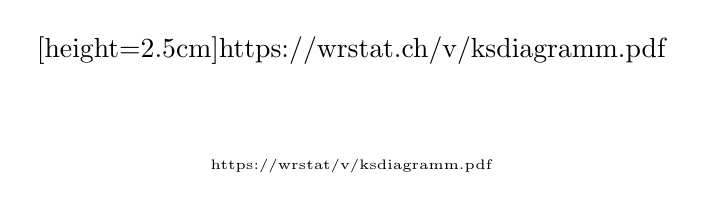
\begin{tikzpicture}[>=latex,thick]
\node at (0,0) {\qrcode[height=2.5cm]{https://wrstat.ch/v/ksdiagramm.pdf}};
\node at (0,-1.25) [below] {\tiny https://wrstat/v/ksdiagramm.pdf};
\end{tikzpicture}}
\end{center}
\vspace*{-20pt}
}
\ifthenelse{\boolean{presentation}}{
\folieninhalt
}{%
\ifthenelse{\boolean{handout}}{
\folieninhalt
}{
\ifthenelse{\boolean{loesungen}}{}{
\begin{center}
\ainput{graph.tex}
\end{center}}}}

\begin{loesung}
In Aufgabe~\ref{80000061} wurden die transformierten Zahlen $F(x_i)$ bereits
berechnet.
Diese werden jetzt auf der $x$-Achse abgetragen und die zugehörige empirische
Verteilungsfunktion gezeichnet.
\begin{center}
\ainput{graph.tex}
\end{center}
\end{loesung}

